\label{sec:exercise_cm_gitlab_usage}

\subsection{Exercise CMGitLabUsage}

\subsubsection*{Description of the M2Go Subgroup Structure}
The subgroup structure in \autoref{fig:screendump_subgroupStructure} only contains the Golang repository.
As the course advances, more repositories will be added to this subgroup.
This repository consists of the following three folders:
\begin{enumerate}
    \item BasicGoProgram/HelloWorld: This folder contains the hello world program introducing the basic Golang syntax
    \item CarRental: This folder contains the CarRental program introducing general Golang features
    \item CarRentalCLI: This folder contains the CarRentalCLI program implementing a more complex version of the CarRental program
\end{enumerate}
Furthermore, there is the .gitignore file and the README.md file.
This structure can be further examined in \autoref{fig:screendump_subsubgroupStructure}.

\begin{figure}[h]
    \centering
    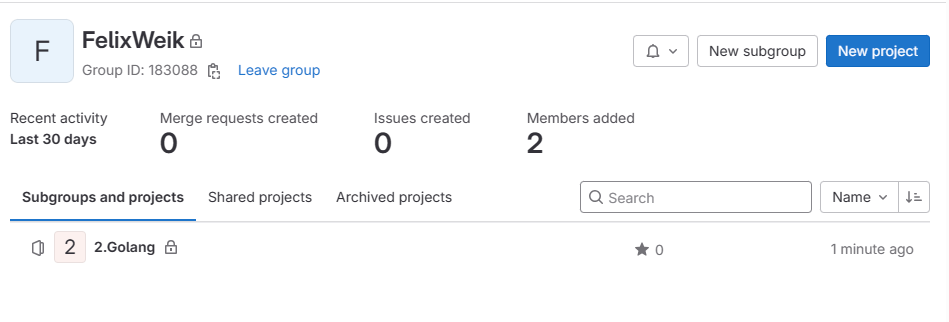
\includegraphics[width=0.8\textwidth]{figures/goLang/golang_personalSubgroupStructure.png}
    \caption{Screendump showing the subgroup structure}
    \label{fig:screendump_subgroupStructure}
\end{figure}

\begin{figure}
    \centering
    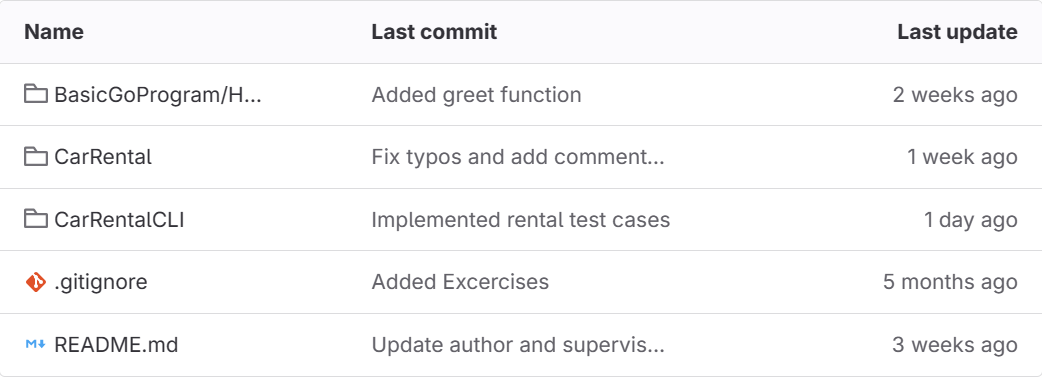
\includegraphics[width=0.8\textwidth]{figures/goLang/golang_personalSubsubgroupStructure.png}
    \caption{Screendump showing the subgroup structure of the Golang folder}
    \label{fig:screendump_subsubgroupStructure}
\end{figure}

\subsubsection*{Repository Cloning Steps}
To clone the repository, the following steps are required:
\begin{enumerate}
    \item Create a Personal Access Token (PAT) on GitLab by going to your Profile Settings and then to Access Tokens
    \item Save the PAT in a safe place
    \item Go to the repository and copy the HTTPS clone URL
    \item Open the WSL2 terminal and navigate to the folder where you want to clone the repository, in my case \texttt{/home/felix/WASA\_M2Go}
    \item Download the repository by running the following command in the terminal: \texttt{git clone <HTTPS clone URL>}
\end{enumerate}

\subsubsection*{First Commit}
After changing the placeholder text in the README.md file, the first commit is done by using the graphical features Visual Studio Code offers.
The commit message shown in \autoref{fig:screendump_readmeCommitMessage} is the following: \texttt{Update author and supervisor in README.md}.

After committing the changes, the changes are pushed to the remote repository, which then becomes visible as shown in \autoref{fig:screendump_readme}.

\begin{figure}[h]
    \centering
    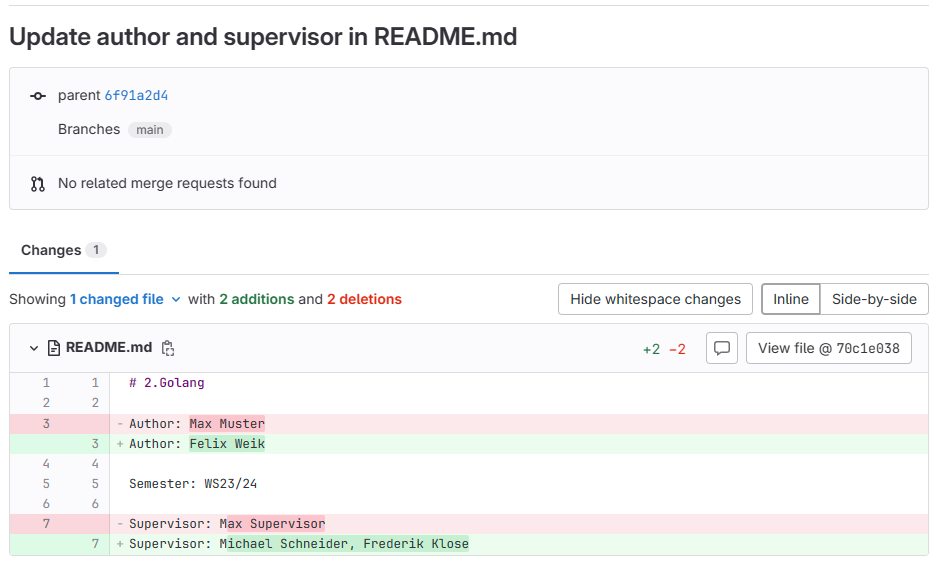
\includegraphics[width=0.8\textwidth]{figures/goLang/golang_screendumpReadmeCommit.png}
    \caption{Screendump showing commit message and the changed files}
    \label{fig:screendump_readmeCommitMessage}
\end{figure}

\begin{figure}[h]
    \centering
    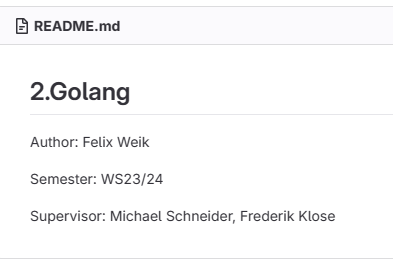
\includegraphics[width=0.5\textwidth]{figures/goLang/golang_screendumpReadme.png}
    \caption{Screendump showing the updated README.md file}
    \label{fig:screendump_readme}
\end{figure}
